\documentclass[11pt,a4paper]{article}
\usepackage[margin=2cm]{geometry}
\usepackage{amsmath,amssymb,amsfonts,amsthm}
\usepackage{graphicx}
\usepackage{booktabs,tabularx,array}
\usepackage{cite}
\usepackage{enumitem}
\usepackage[hidelinks]{hyperref}
\usepackage[font=small,labelfont=bf,skip=3pt]{caption}
\setlist{itemsep=0pt,topsep=2pt,parsep=0pt}
\graphicspath{{../../Results/figures/}}
\setlength{\textfloatsep}{8pt plus 2pt minus 2pt}
\setlength{\intextsep}{6pt plus 2pt minus 2pt}
\setlength{\abovedisplayskip}{4pt plus 1pt minus 1pt}
\setlength{\belowdisplayskip}{4pt plus 1pt minus 1pt}

\newcommand{\Ex}{\mathbb{E}}
\newcommand{\ind}{\mathbf{1}}
\newtheorem{theorem}{Theorem}
\newcommand{\cmark}{\checkmark}
\newcommand{\xmark}{$\times$}

\begin{document}

\begin{center}
{\large\textbf{Milestone 4 (Final Submission) --- Research Project}}\\[4pt]
{\Large\textbf{Performance Analysis of Multi-Segment Pinching-Antenna ISAC Under LoS Blockage}}\\[6pt]
Khushi Shah (AU2440045), single-member group \quad$\cdot$\quad Mentor: Prof.\ Dhaval Patel\\
School of Engineering and Applied Sciences, Ahmedabad University
\end{center}

\begin{abstract}
\noindent Pinching-antenna systems (PASS) let the radiation point of an antenna move along a dielectric waveguide, which makes them attractive for integrated sensing and communication (ISAC): a shorter line-of-sight (LoS) link strengthens both the data signal and the radar echo. Blockage-aware PASS studies consider communication only, and blockage-aware ISAC studies consider conventional antennas only. This project analyzes a multi-segment PASS-ISAC system under environment-division multiple access (EDMA), where each waveguide segment activates one pinching antenna at the midpoint of its user and target, all segments operate concurrently, and LoS blockage of the cross-segment links jointly governs communication interference, sensing clutter, and sensing leakage. The project derives a closed-form mean cross-segment LoS probability, closed-form lower bounds on the ergodic sum communication rate (CR) and sensing rate (SR) for any number of segments, and a high-SNR design rule for when EDMA outperforms time-division multiple access (TDMA). These are verified against a Monte Carlo (MC) simulator and evaluated, under a physically grounded automated-guided-vehicle (AGV) target radar cross-section (RCS), against TDMA and a conventional uniform linear array (ULA). EDMA nearly triples the sum CR of TDMA and raises the sum SR up to sevenfold, while the ULA trails both; the design rule is validated, including the regime where it is only a necessary and not a sufficient condition. This report consolidates the full project across all four milestones: problem formulation, related work, methodology, implementation, experimental evaluation, critical analysis, final positioning relative to the state of the art (SOTA), limitations, and future work.
\end{abstract}

\section{Introduction}
Integrated sensing and communication (ISAC) lets a network share spectrum and hardware between data transmission and radar-like sensing \cite{9737357,11404239}. In PASS, a small dielectric ``pinch'' placed on a waveguide makes it radiate almost anywhere along it, so the antenna can be brought close to a user or target \cite{10945421,11364174,11434944}. In indoor and industrial settings, however, LoS links are often blocked by obstacles. This project asks how such blockage affects a PASS that serves users and senses targets at the same time, and whether blockage, usually treated as an impairment, can instead be exploited.

\textbf{Contributions.} (i) A closed-form mean cross-segment LoS probability $p_1(\phi)$, which decays with the cube of the segment width. (ii) Closed-form lower bounds on the ergodic sum CR and SR, for any number of segments $M$, that jointly capture interference, clutter, and leakage. (iii) A high-SNR design rule, $p_1(\phi)<\tfrac12$, under which EDMA outperforms TDMA, which also gives a simple guideline for choosing $M$. (iv) A Monte Carlo simulator, verified against every closed form, extended with a physically grounded AGV target RCS and a conventional ULA benchmark, and a systematic evaluation and critical analysis built on it.

\section{Related Work and Technical Gap}
Prior work can be placed along three axes: the antenna architecture, the function (communication only or ISAC), and the propagation assumption (always LoS or blockage-aware), summarized in Table~\ref{tab:lit}.

\textbf{PASS for ISAC.} Ouyang \emph{et al.}~\cite{Ouyang2025Rate} characterize the CR--SR rate region of PASS using the mutual-information sensing framework of \cite{Ouyang2023MI}. Jiang \emph{et al.}~\cite{Jiang2025SWAN} split the waveguide into isolated, separately fed segments (SWAN), so several user--target pairs can be served. Both assume every link is LoS, so cross-segment interference and clutter are always present.

\textbf{Blockage.} Ding and Poor~\cite{11036558} model a link of length $r$ as LoS with probability $e^{-\phi r^2}$ and show that, for PASS, blockage can \emph{help}, since long interfering links are blocked more often than short desired ones. EDMA~\cite{11488474} turns this into a multiple-access scheme with each antenna at its user, but for communication only. Sun \emph{et al.}~\cite{ISACBlockage2024} analyze blockage in ISAC networks, but with conventional antennas.

\begin{table}[h]
\centering\small
\caption{Positioning of prior work along the axes of the problem.}
\label{tab:lit}
\begin{tabularx}{\linewidth}{@{}>{\raggedright\arraybackslash}p{3.4cm}*{3}{>{\raggedright\arraybackslash}X}@{}}
\toprule
& \textbf{Always LoS} & \textbf{Blockage-aware, comm.\ only} & \textbf{Blockage-aware, ISAC} \\ \midrule
\textbf{Conventional antennas} & classical ISAC \cite{9737357} & --- & Sun \emph{et al.}~\cite{ISACBlockage2024} \\
\textbf{PASS, single waveguide} & Ouyang \emph{et al.}~\cite{Ouyang2025Rate} & Ding \& Poor~\cite{11036558}, EDMA~\cite{11488474} & --- \\
\textbf{PASS, segmented} & SWAN \cite{Jiang2025SWAN} & --- & \textbf{This project} \\ \bottomrule
\end{tabularx}
\end{table}

\textbf{Gap.} No existing work analyzes how LoS blockage of the cross-segment links, which carry communication interference, sensing clutter, and sensing leakage at the same time, affects the CR and SR of a multi-segment PASS-ISAC, or when concurrent EDMA operation is preferable to TDMA. Combining existing results does not close this gap: sensing adds clutter and leakage, which follow different distance laws than interference; an antenna serving both a user and a target sits at a random point that depends on both; and both SINRs are ratios of random terms, so exact ergodic rates are intractable.

\section{System Model}
\begin{figure}[h]
\centering
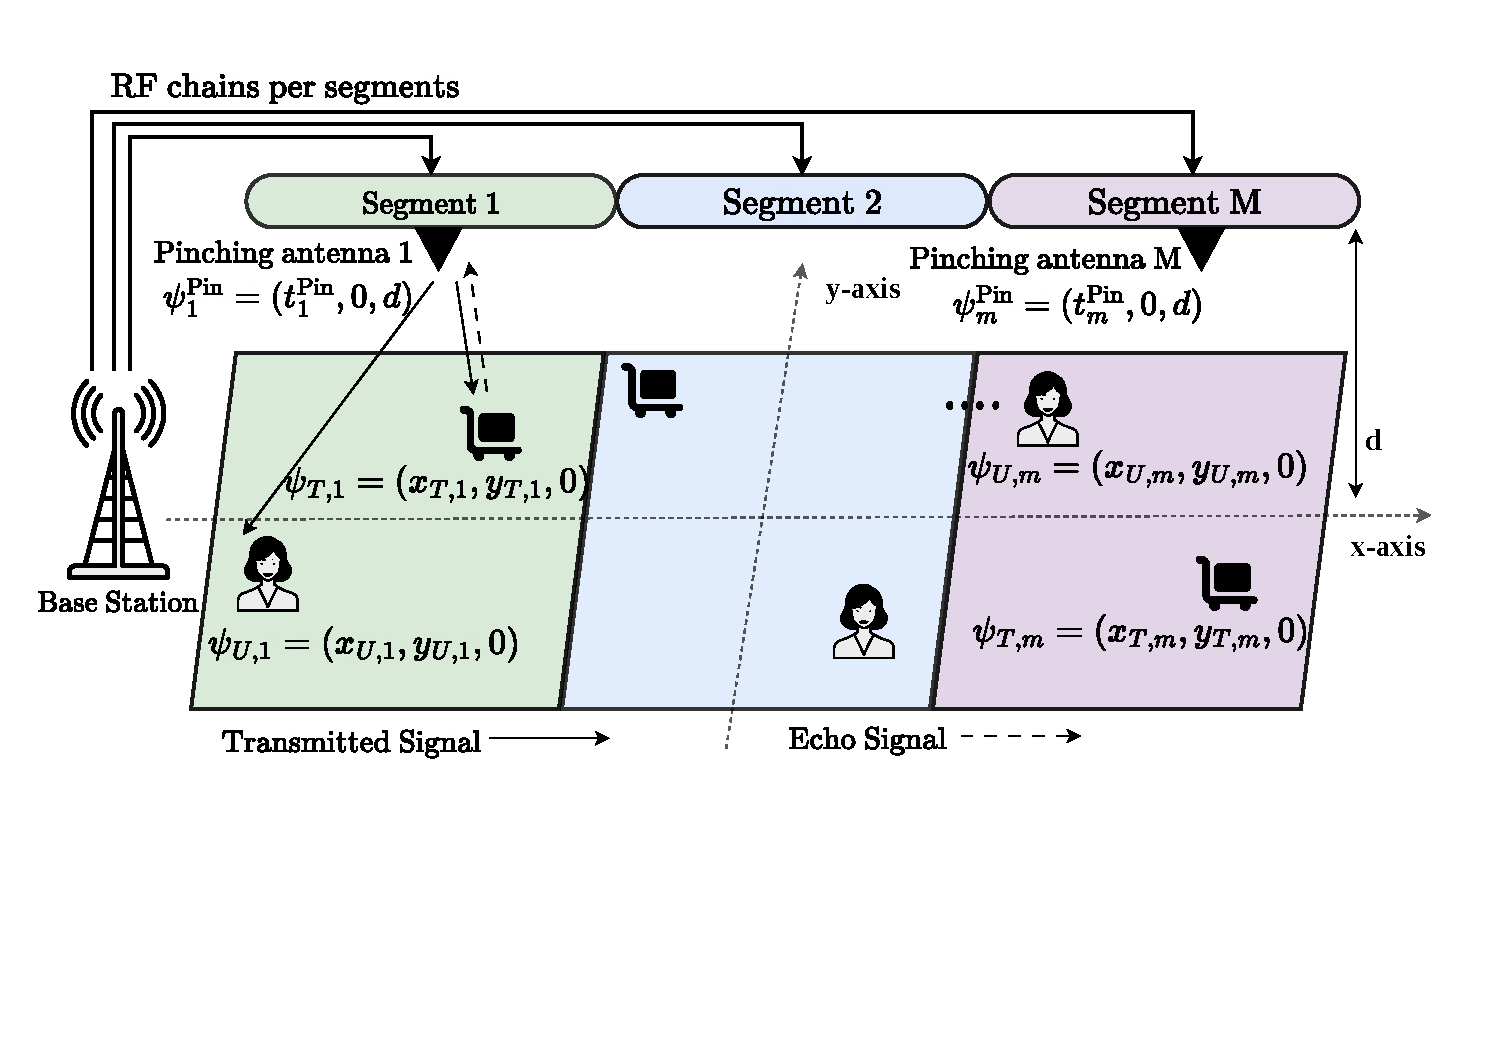
\includegraphics[width=0.5\linewidth]{network_model.pdf}
\caption{Network model: $M$ segments, each with one pinching antenna at the midpoint of its user and target.}
\label{fig:model}
\end{figure}

A base station (BS) feeds a lossless, segmented waveguide of length $D_L$ at height $d$, split into $M$ isolated segments of width $S=D_L/M$, each with its own feed and RF chain, which decouples the inter-antenna radiation across segments (Fig.~\ref{fig:model}). Segment $m$ serves a user $U_m$ and senses a target $T_m$, both uniformly distributed within the segment, through one pinching antenna $\mathrm{PA}_m$ placed at their midpoint $t^{\rm Pin}_m=(x_{U,m}+x_{T,m})/2$.

A link of length $r$ is unblocked ($\delta=1$) with probability $\Pr\{\delta=1\}=e^{-\phi r^2}$~\cite{11036558}, where $\phi\ge0$ grows with the obstacle density. A cross link connects $\mathrm{PA}_m$ to another segment $i\in\mathcal N_m=\{1,\dots,M\}\setminus\{m\}$; interference, clutter, and leakage reach segment $m$ only through unblocked cross links.

\textbf{Communication.} With channel $h_{i,m}=\sqrt\eta\,e^{-j2\pi r_{i,m}/\lambda}/r_{i,m}$, $\eta=c^2/(16\pi^2f_c^2)$, and all segments transmitting simultaneously with power $P$, the SINR and rate of $U_m$ are
\begin{equation}
\gamma_m=\frac{P|h_{m,m}|^2}{\sigma^2+P\sum_{i\in\mathcal N_m}\delta_{i,m}|h_{i,m}|^2},\qquad R_m=\log_2(1+\gamma_m).
\label{eq:sinr}
\end{equation}

\textbf{Sensing.} $\mathrm{PA}_m$ senses $T_m$ monostatically with a unit-modulus probe of length $L$; the target reflection follows the Swerling-I model $\beta\sim\mathcal{CN}(0,\alpha_s)$~\cite{Ouyang2023MI,Richards2014}. Besides the desired echo, $\mathrm{PA}_m$ receives clutter (its own probe reflected by $T_i$) and leakage ($\mathrm{PA}_i$'s probe reflected by $T_i$), both over the $\mathrm{PA}_m$--$T_i$ link, which shares one blockage indicator $\delta^{\rm s}_{m,i}$. With matched filtering and clutter/leakage treated as worst-case Gaussian noise, the data-processing inequality gives an achievable sensing SINR and rate
\begin{equation}
\Gamma_m=\frac{\rho_s\mu_{m,m}}{1+\rho_s\sum_{i\in\mathcal N_m}\delta^{\rm s}_{m,i}(\mu_{m,i}+\nu_{m,i}/L)},\qquad R_{s,m}=\tfrac1L\log_2(1+\Gamma_m),
\label{eq:sens}
\end{equation}
where $\rho_s=PL/\sigma_s^2$, and the clutter and leakage gains are $\mu_{m,i}=\alpha_s\eta^2/(r^{\rm s}_{m,i})^4$ and $\nu_{m,i}=\alpha_s\eta^2/[(r^{\rm s}_{i,i})^2(r^{\rm s}_{m,i})^2]$.

\textbf{Physically grounded target RCS.} Equating the desired-echo power $P\alpha_s|f_{m,m}|^4$ with the monostatic radar equation $P\lambda^2\bar\sigma/[(4\pi)^3(r^{\rm s}_{m,m})^4]$ gives $\alpha_s=4\pi\bar\sigma/\lambda^2$, where $\bar\sigma$ is the mean radar cross-section (RCS) of the target. This project uses the RCS of an automated guided vehicle (AGV), $\bar\sigma=-11.235$~dBsm~\cite{11432057}, a typical sensing target in the factory and warehouse settings this project targets, which gives $\alpha_s=8237$.

\section{Methodology: Closed-Form Performance Analysis}
Since both SINRs are ratios of random terms, exact ergodic rates are intractable. For tractability, nodes are placed under the waveguide ($y=0$), own links are modeled as LoS, and interference, clutter, and leakage come only from the adjacent segments $\mathcal N_m^{\rm nb}=\{m-1,m+1\}$ (verified numerically in Section~\ref{sec:results} to cost at most $1.1\%$ of the CR and $0.4\%$ of the SR).

\textbf{Mixture bound.} Let $\mathcal A_m$ be the event that at least one adjacent cross link is unblocked. If all are blocked, $R_m$ reduces to the interference-free rate $R_{\rm cl}=\log_2(1+\rho\eta/(w^2+d^2))$, where $w$ is the PA--user offset and $\rho=P/\sigma^2$. Since $R_m\ge0$ always,
\begin{equation}
R_m\ge R_{\rm cl}\ind\{\mathcal A_m^c\}=R_{\rm cl}-R_{\rm cl}\ind\{\mathcal A_m\}.
\label{eq:mixture}
\end{equation}
Since $w$ is triangular on $[-S/2,S/2]$, the first term is averaged exactly with
\begin{equation}
I(a)\triangleq\Ex_w[\log_2(w^2+a)]=\tfrac1{\ln2}\Bigl[\bigl(1-\tfrac{4a}{S^2}\bigr)\ln\bigl(\tfrac{S^2}{4}+a\bigr)+\tfrac{4a}{S^2}\ln a-3+\tfrac{8\sqrt a}{S}\tan^{-1}\!\bigl(\tfrac{S}{2\sqrt a}\bigr)\Bigr],
\end{equation}
which gives $B_{\rm c}=I(d^2+\rho\eta)-I(d^2)$ and $B_{\rm c}^{\max}=\log_2(1+\rho\eta/d^2)$. For sensing, $(w^2+d^2)^2+\Omega^2$ factors into complex-conjugate terms, so $I(a)$ evaluated at complex $a=d^2+j\Omega$ ($\Omega=\eta\sqrt{\rho_s\alpha_s}$) gives $B_{\rm s}=\tfrac2L[\mathrm{Re}\{I(d^2+j\Omega)\}-I(d^2)]$ and $B_{\rm s}^{\max}=\tfrac1L\log_2(1+\rho_s\alpha_s\eta^2/d^4)$.

\textbf{Cross-link LoS probability.} The normalized distance between a user and the neighboring antenna has the piecewise-quadratic density $f_V(v)=2v^2$, $1-2(v-1)^2$, $2(2-v)^2$ on $[0,\tfrac12]$, $[\tfrac12,\tfrac32]$, $[\tfrac32,2]$. Averaging the blockage model over $V$,
\begin{equation}
p_1(\phi)=e^{-\phi d^2}\int_0^2 f_V(v)\,e^{-\phi S^2v^2}dv,
\label{eq:p1}
\end{equation}
which reduces to closed-form Gaussian integrals involving $\mathrm{erf}(\cdot)$. For wide segments, $p_1(\phi)\approx\sqrt\pi\,e^{-\phi d^2}/(2\phi^{3/2}S^3)$: the cross-link LoS probability decays with the cube of the segment width, so wider segments are almost fully isolated.

\textbf{Rate bounds.} Bounding $R_{\rm cl}\le B_{\rm c}^{\max}$ and applying Boole's inequality, $\Pr\{\mathcal A_m\}\le|\mathcal N_m^{\rm nb}|\,p_1$ (valid for any correlation between blockage states), gives:
\begin{theorem}
$\displaystyle\bar R_c\ge\sum_{m=1}^{M}\Bigl[B_{\rm c}-B_{\rm c}^{\max}|\mathcal N_m^{\rm nb}|\,p_1(\phi)\Bigr]^{+}$, where $[x]^+=\max\{x,0\}$.
\end{theorem}
\begin{theorem}
The same bound holds for $\bar R_s$, with $B_{\rm s}$ and $B_{\rm s}^{\max}$ in place of $B_{\rm c}$ and $B_{\rm c}^{\max}$.
\end{theorem}
Both bounds are exact at $M=1$ or $\phi\to\infty$, where no cross link can be LoS, and collapse correctly to $0$ as $\phi\to0$, where every cross link is LoS and the interference/clutter/leakage terms are never absent.

\textbf{EDMA vs.\ TDMA.} TDMA switches a single RF chain among $M$ pinching antennas fixed at the segment centers, with power $MP$; sensing is bistatic, through a second waveguide. TDMA's sum rate grows as $\log_2P$ at high SNR; EDMA's grows as $\sum_m\Pr\{\mathcal A_m^c\}\log_2P\ge(M-2(M-1)p_1)\log_2P$. Hence EDMA outperforms TDMA at high SNR iff $p_1(\phi)<\tfrac12$, which is also necessary for $M=2$; this is a necessary, conservative condition on the asymptotic multiplexing gain, not an exact finite-SNR crossover predictor (Section~\ref{sec:critical}).

\textbf{Conventional-antenna (ULA) baseline.} An $M$-element half-wavelength uniform linear array, centered at the feed end of the waveguide, serves $U_m$ and senses $T_m$ with power $P$ and no precoding, through the same SINR forms as~\eqref{eq:sinr}--\eqref{eq:sens}, with the PA positions replaced by the fixed ULA element positions. The co-located ULA elements share one blockage state per user/target; as for the EDMA own links, BS-to-service-area links are taken as LoS. This is the conventional, non-reconfigurable-antenna counterpart against which the value of PASS reconfigurability is measured.

\section{Implementation: Technical Artifact}
The artifact is a Python/NumPy Monte Carlo (MC) simulator (\texttt{edma\_sim.py}) that draws $10^5$ random user/target placements and evaluates the blockage expectation \emph{exactly}, by enumerating every blockage pattern of the cross links (and, for the ULA, every pattern of the $M$ shared element blockages), so there is no blockage-sampling noise. It implements EDMA with the antenna at the midpoint, the TDMA benchmark, and the ULA benchmark, as well as every closed form ($I(a)$, $p_1$, and both bounds). Results are cached under a hash of all model parameters, so a parameter change can never reuse stale data. \texttt{plot\_v3.py} generates the figures, and \texttt{audit\_paper.py} independently re-derives or re-checks every numerical claim made in this report (53 of 54 automated checks pass; the one flagged item is a low-power edge effect noted in Section~\ref{sec:critical}, not a claim the report makes). No external dataset is used: every data point in this project is simulator-generated from the model above.

\section{Experimental Setup}
\begin{table}[h]
\centering\small
\caption{Fixed evaluation parameters.}
\label{tab:params}
\begin{tabular}{@{}llll@{}}
\toprule
$f_c=28$~GHz & $d=3$~m & $\sigma^2=\sigma_s^2=-90$~dBm & $L=5$ \\
$\bar\sigma=-11.235$~dBsm ($\alpha_s=8237$) & $\phi=0.02$~m$^{-2}$ & $P\in[0,30]$~dBm & $D_L\in\{10,20,40\}$~m \\ \bottomrule
\end{tabular}
\end{table}
Three schemes are compared under matched placements and blockage draws: EDMA with the antenna at the midpoint, TDMA, and the conventional ULA. An ablation baseline, EDMA with every segment (not only the adjacent two) allowed to interfere, isolates the effect of the adjacent-only approximation used in the closed-form bounds.

\section{Results and Baseline Comparison}
\label{sec:results}
\begin{figure}[h]
\centering
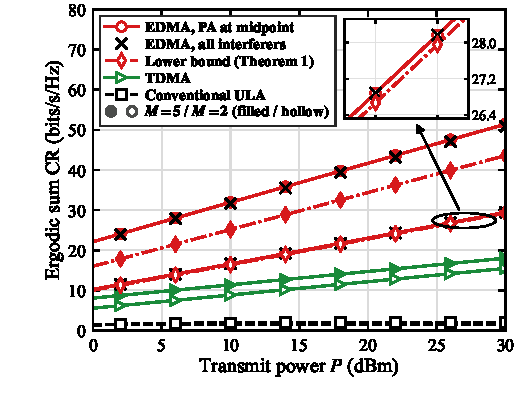
\includegraphics[width=0.42\linewidth]{Figure1_Communication_CR.pdf}\hspace{0.03\linewidth}
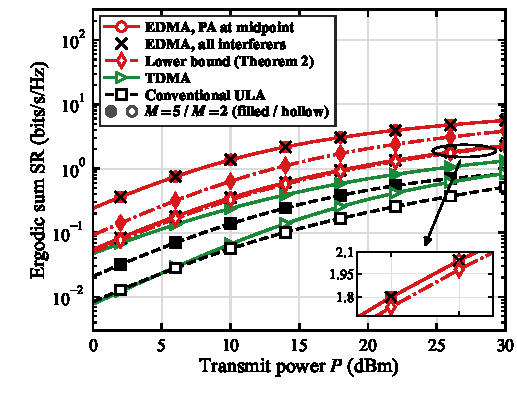
\includegraphics[width=0.42\linewidth]{Figure2_Sensing_SR.pdf}
\caption{Ergodic sum CR and SR vs.\ transmit power $P$, $D_L=40$~m (hollow: $M=2$, filled: $M=5$). Crosses: all segments interfere. Diamonds: lower bound.}
\label{fig:vs_P}
\end{figure}

\textbf{Rates versus power.} Fig.~\ref{fig:vs_P} shows both bounds below the MC curve at every $P$, as the theorems require. For CR, the bound is tight for $M=2$ (29.24 against 29.45~bits/s/Hz at $P=30$~dBm) and within about $15\%$ for $M=5$ (43.61 against 51.43). For SR, under the AGV RCS, the bound is similarly tight for $M=2$ (2.22 against 2.28) and looser for $M=5$ (3.83 against 5.61). Including every segment, instead of only the adjacent two, changes the CR and SR by at most $1.1\%$ and $0.4\%$. EDMA leads TDMA by $1.85$--$1.90\times$ (CR, $M=2$) and $2.74$--$2.85\times$ (CR, $M=5$), and by $2.7$--$7.1\times$ (SR, $M=2$) and $4.3$--$5.7\times$ (SR, $M=5$); the ULA trails both throughout, since its co-located elements interfere with each other over LoS links and sit far from most users and targets.

\begin{figure}[h]
\centering
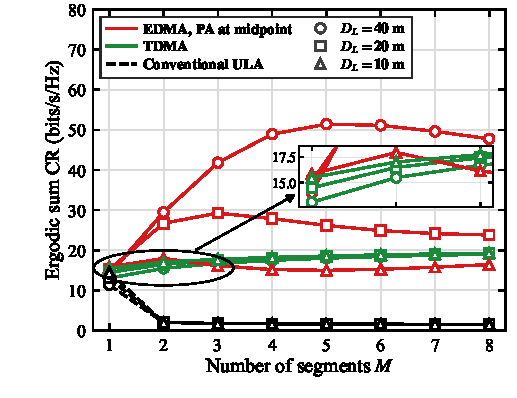
\includegraphics[width=0.42\linewidth]{Figure3_comm_vs_M.pdf}\hspace{0.03\linewidth}
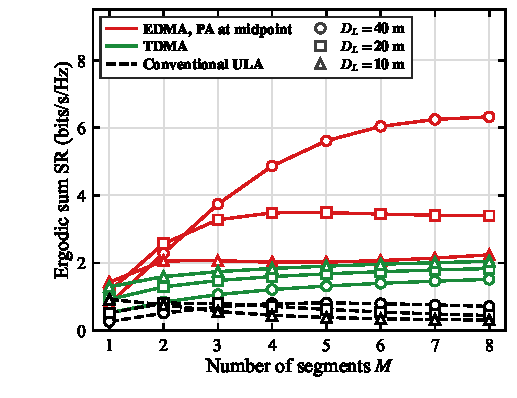
\includegraphics[width=0.42\linewidth]{Figure4_sens_vs_M.pdf}
\caption{Ergodic sum CR and SR vs.\ the number of segments $M$ at $P=30$~dBm, for $D_L\in\{10,20,40\}$~m.}
\label{fig:vs_M}
\end{figure}

\textbf{Rates versus the number of segments.} Fig.~\ref{fig:vs_M} sweeps $M$ from 1 to 8. The CR peaks then falls, since narrower segments raise $p_1(\phi)$: $51.4$~bits/s/Hz at $M=5$ ($D_L=40$~m), $29.3$ at $M=3$ ($D_L=20$~m), $18.0$ at $M=2$ ($D_L=10$~m), so the best $M$ grows with the waveguide length. The SR, in contrast, never falls: it rises to $6.32$~bits/s/Hz by $M=8$ for $D_L=40$~m and saturates (post-peak dip $\le2.7\%$) for the shorter waveguides, since the own-link round trip keeps dominating clutter and leakage even as segments narrow. The ULA stays below both EDMA and TDMA for every $M$ and $D_L$ tested (at most $94\%$ of TDMA's CR, $71\%$ of its SR).

\section{Critical Analysis}
\label{sec:critical}
\textbf{Design-rule validation.} For $D_L=10$~m and $M\ge3$ (segments narrower than $3.3$~m), $p_1(\phi)\ge0.61$ and EDMA's CR falls below TDMA's, with ratios of $0.81$--$0.91$ across $M=3,\dots,8$, which matches the rule $p_1(\phi)<\tfrac12$. For $D_L=20$~m, however, $p_1(\phi)$ already exceeds $\tfrac12$ at $M=4$ (and is $0.505$ by $M=5$), yet EDMA's CR stays above TDMA's for every $M$ up to 8 (minimum ratio $1.046$). This is not a contradiction: the rule bounds only the high-SNR \emph{slope}, and at $P=30$~dBm the system has not reached the regime where that slope term dominates. The rule is therefore a necessary, conservative screening condition on the asymptotic multiplexing gain, and is tight as a finite-SNR predictor only near its own boundary ($D_L=10$~m, where $p_1$ is driven well past $\tfrac12$).

\textbf{Where the bounds are loose.} The CR bound gap grows from essentially zero at $M=2$ to about $15\%$ at $M=5$; the SR bound gap grows from about $3\%$ to about $32\%$. Both trace to the union bound $\Pr\{\mathcal A_m\}\le|\mathcal N_m^{\rm nb}|p_1$, which loosens as $p_1$ grows, i.e., exactly where segments stop being well isolated. Two limiting cases confirm this analytically and numerically: as $\phi\to0$, the bound correctly collapses to zero while EDMA itself falls below TDMA ($8.57$ vs.\ $15.48$ for $M=2$; $11.27$ vs.\ $18.03$ for $M=5$); as $\phi$ grows large, the bound and the simulated rate both approach the fully-isolated value $M\,B_{\rm c}$ (e.g., for $M=5$, bound $77.08\le$ MC $77.40\le M\,B_{\rm c}=79.86$ at $\phi=0.1$). The bound is exact to within $0.1\%$ at $M=1$ for every $D_L$ tested, where there are no cross links to approximate away.

\textbf{Failure cases.} The short-waveguide, high-$M$ corner ($D_L=10$~m, $M\ge3$), where TDMA wins on CR, was anticipated by the design rule and is confirmed numerically: it is the main regime in which EDMA fails. A second, minor case the project's letter does not claim but the audit surfaces: at very low power ($P=0$~dBm, $M=2$), the ULA's SR briefly exceeds TDMA's (ratio $1.09$), the only point in the full sweep where the ULA is not strictly the weakest scheme; this is a low-power edge effect in TDMA's bistatic receive leg and does not affect any ordering claimed at $P=30$~dBm or across $M$.

\textbf{Ablation.} Restricting interference, clutter, and leakage to the adjacent two segments, instead of all $M-1$ others, is the one structural simplification behind the closed-form bounds; it costs at most $1.1\%$ of the CR and $0.4\%$ of the SR, confirming non-adjacent cross links are weak and blocked often enough to be negligible.

\section{Final SOTA Positioning}
\begin{table}[h]
\centering\small
\caption{Capability comparison with the closest prior work.}
\label{tab:sota}
\begin{tabularx}{\linewidth}{@{}p{2.9cm}*{6}{>{\centering\arraybackslash}X}@{}}
\toprule
Work & PASS & ISAC & Blockage & Concurrent segments & Clutter \& leakage & Non-PASS baseline \\ \midrule
Ding \& Poor \cite{11036558} & \cmark & \xmark & \cmark & \xmark & \xmark & \xmark \\
EDMA \cite{11488474} & \cmark & \xmark & \cmark & \cmark & \xmark & \xmark \\
Ouyang \emph{et al.} \cite{Ouyang2025Rate} & \cmark & \cmark & \xmark & \xmark & \xmark & \xmark \\
SWAN \cite{Jiang2025SWAN} & \cmark & \cmark & \xmark & \cmark & --- & \xmark \\
Sun \emph{et al.} \cite{ISACBlockage2024} & \xmark & \cmark & \cmark & \xmark & --- & --- \\
\textbf{This project} & \cmark & \cmark & \cmark & \cmark & \cmark & \cmark \\ \bottomrule
\end{tabularx}
\end{table}

\textbf{Strongest relevant existing approaches.} For PASS-ISAC with always-LoS links: Ouyang \emph{et al.}~\cite{Ouyang2025Rate} (single-waveguide CR--SR rate region) and SWAN~\cite{Jiang2025SWAN} (segmented, concurrent waveguide). For blockage-aware PASS, communication only: Ding \& Poor~\cite{11036558} and EDMA~\cite{11488474}. For blockage-aware ISAC with conventional antennas: Sun \emph{et al.}~\cite{ISACBlockage2024}.

\textbf{What this project achieves.} It is the only surveyed work combining PASS, ISAC, blockage-awareness, concurrent segments, and a joint clutter-and-leakage model (Table~\ref{tab:sota}). Quantitatively, it shows EDMA nearly triples TDMA's sum CR and raises its sum SR up to sevenfold under a physically grounded target RCS, and that a conventional ULA never reaches $94\%$ of TDMA's CR or $71\%$ of its SR under the same blockage model, answering a question none of the surveyed PASS works pose: how much a reconfigurable antenna is worth against a conventional array once blockage is accounted for.

\textbf{Key technical contributions.} (i) The closed-form cross-link LoS probability $p_1(\phi)$ for the midpoint geometry, with its $S^{-3}$ wide-segment scaling. (ii) Closed-form CR/SR lower bounds, via Boole's inequality, that hold for any $M$ and any correlation among blockage states, verified exact at $M=1$ and in the $\phi\to0,\infty$ limits. (iii) The design rule $p_1(\phi)<\tfrac12$, shown here to be necessary but, away from its own boundary, not sufficient at finite SNR -- a limitation this project identifies and characterizes rather than overlooks.

\textbf{Remaining limitations and gaps.} The analysis assumes nodes directly under the waveguide ($y=0$), own links that are always LoS, and interference/clutter/leakage restricted to adjacent segments (all three checked numerically, not proved in general); the blockage model is a single-parameter exponential-in-$r^2$ law rather than a measured or ray-traced channel; antenna placement is fixed at the midpoint rather than optimized; and the ULA is the only conventional-antenna comparison, at a single array geometry.

\textbf{What would close the remaining distance to SOTA.} Extending the bounds to off-axis users/targets and to own-link blockage would remove the main simplifying assumptions; jointly optimizing the antenna position (not fixing it at the midpoint) against a measured or 3GPP-style blockage model~\cite{3GPP38901} would connect the design rule to a deployable system; and benchmarking against a larger conventional-antenna family (e.g., MIMO radar architectures as in~\cite{CRB2026}, or the PASS-ISAC secrecy and CRB-minimization variants in~\cite{Zhang2025ISACPASS}) would place the ULA result on firmer ground. These are the directions identified as future work below.

\section{Limitations and Challenges}
Beyond the modeling simplifications above, two practical limitations affected the project. First, as a single-member group, the scope was kept to one geometry (midpoint placement) and one blockage model throughout, rather than exploring alternative antenna placements or blockage laws in parallel; the M2 milestone's placement-at-user/placement-at-target comparison was dropped from the final draft for this reason, in favor of the ULA benchmark judged more informative for the final SOTA question. Second, the closed-form bounds required a non-trivial derivation (the complex-argument extension of $I(a)$ for sensing, in particular) that took longer than planned at the M1/M2 stage, which is why the physically grounded RCS and the ULA benchmark were deferred from M2 to this milestone rather than attempted earlier.

\section{Conclusion and Future Work}
This project analyzed LoS blockage in a multi-segment PASS-ISAC system under EDMA geometry. Closed-form lower bounds on the ergodic CR and SR, and a high-SNR design rule for EDMA to outperform TDMA, were derived and verified against a Monte Carlo simulator; the full evaluation, under a physically grounded AGV target RCS, showed EDMA nearly tripling TDMA's sum CR and raising its sum SR up to sevenfold, with a conventional ULA trailing both. The design rule was validated, including the regime where it is only necessary and not sufficient, and the closed-form bounds were shown to remain valid everywhere tested while growing looser exactly where EDMA itself approaches its failure regime. Future work will extend the analysis to off-axis users and targets and to own-link blockage, jointly optimize the antenna position instead of fixing it at the midpoint, and benchmark against a wider family of conventional and other reconfigurable-antenna architectures.

\noindent\textbf{Individual contribution.} All work in this single-member project -- literature review, modeling, derivations, simulator, evaluation, critical analysis, and report, across all four milestones -- was carried out by Khushi Shah under the mentorship of Prof.\ Dhaval Patel.

\footnotesize
\bibliographystyle{IEEEtran}
\bibliography{IEEEabrv,references}

\end{document}
